\frontmatter
\pagestyle{plain}
\pagestyle{empty}
\begin{center}

\vspace{1.5cm}
{\Huge \bfseries \ttitle}

\vspace{1.5cm}
\IfFileExists{imgs/logo.pdf}{
\begin{figure}[h]
  \centering
  
\includegraphics[width=2.5in, height=2.5in]{imgs/logo.pdf}
\end{figure}
}{
\vspace{1.8in}
}

\vspace{2cm}

{\LARGE
\begin{tabular}{ll}
\textbf{Utkarsh Kumar} & 23114101 \\
\end{tabular}}

{\Large
\vspace{0.8cm}
\deptname\\
\univname\\
\addressname\\
\vspace{2.8cm}
\reptype\\
\vspace{1.0cm}
April, 2026}

\end{center}

\clearpage

\hypersetup{linkcolor=blue}
\renewcommand\arraystretch{1.1}

\mainmatter
\pagestyle{thesis}

\chapter*{Competition - IIT Pokerbots 2026}

\begin{figure}[htbp]
\centering
\begin{minipage}{0.45\textwidth}
I participated in IIT Pokerbots 2026 a pan-IIT competition which focused on building autonomous agents for decision-making. I developed a poker-playing bot for the custom heads-up game \textit{Sneak Peek Hold'em} where players make strategic decisions under incomplete information using probability and game theory.

\vspace{1em}

I achieved \textbf{Rank 35}, demonstrating strong performance and an effective algorithmic approach. The competition required bots to compete through multiple automated rounds as their goal was to increase total chip winnings. It was conducted from \href{https://www.iitpokerbots.in/dashboard/timeline}{28 February to 7 March 2026}. 
\end{minipage}
\hfill
\begin{minipage}{0.5\textwidth}
\centering
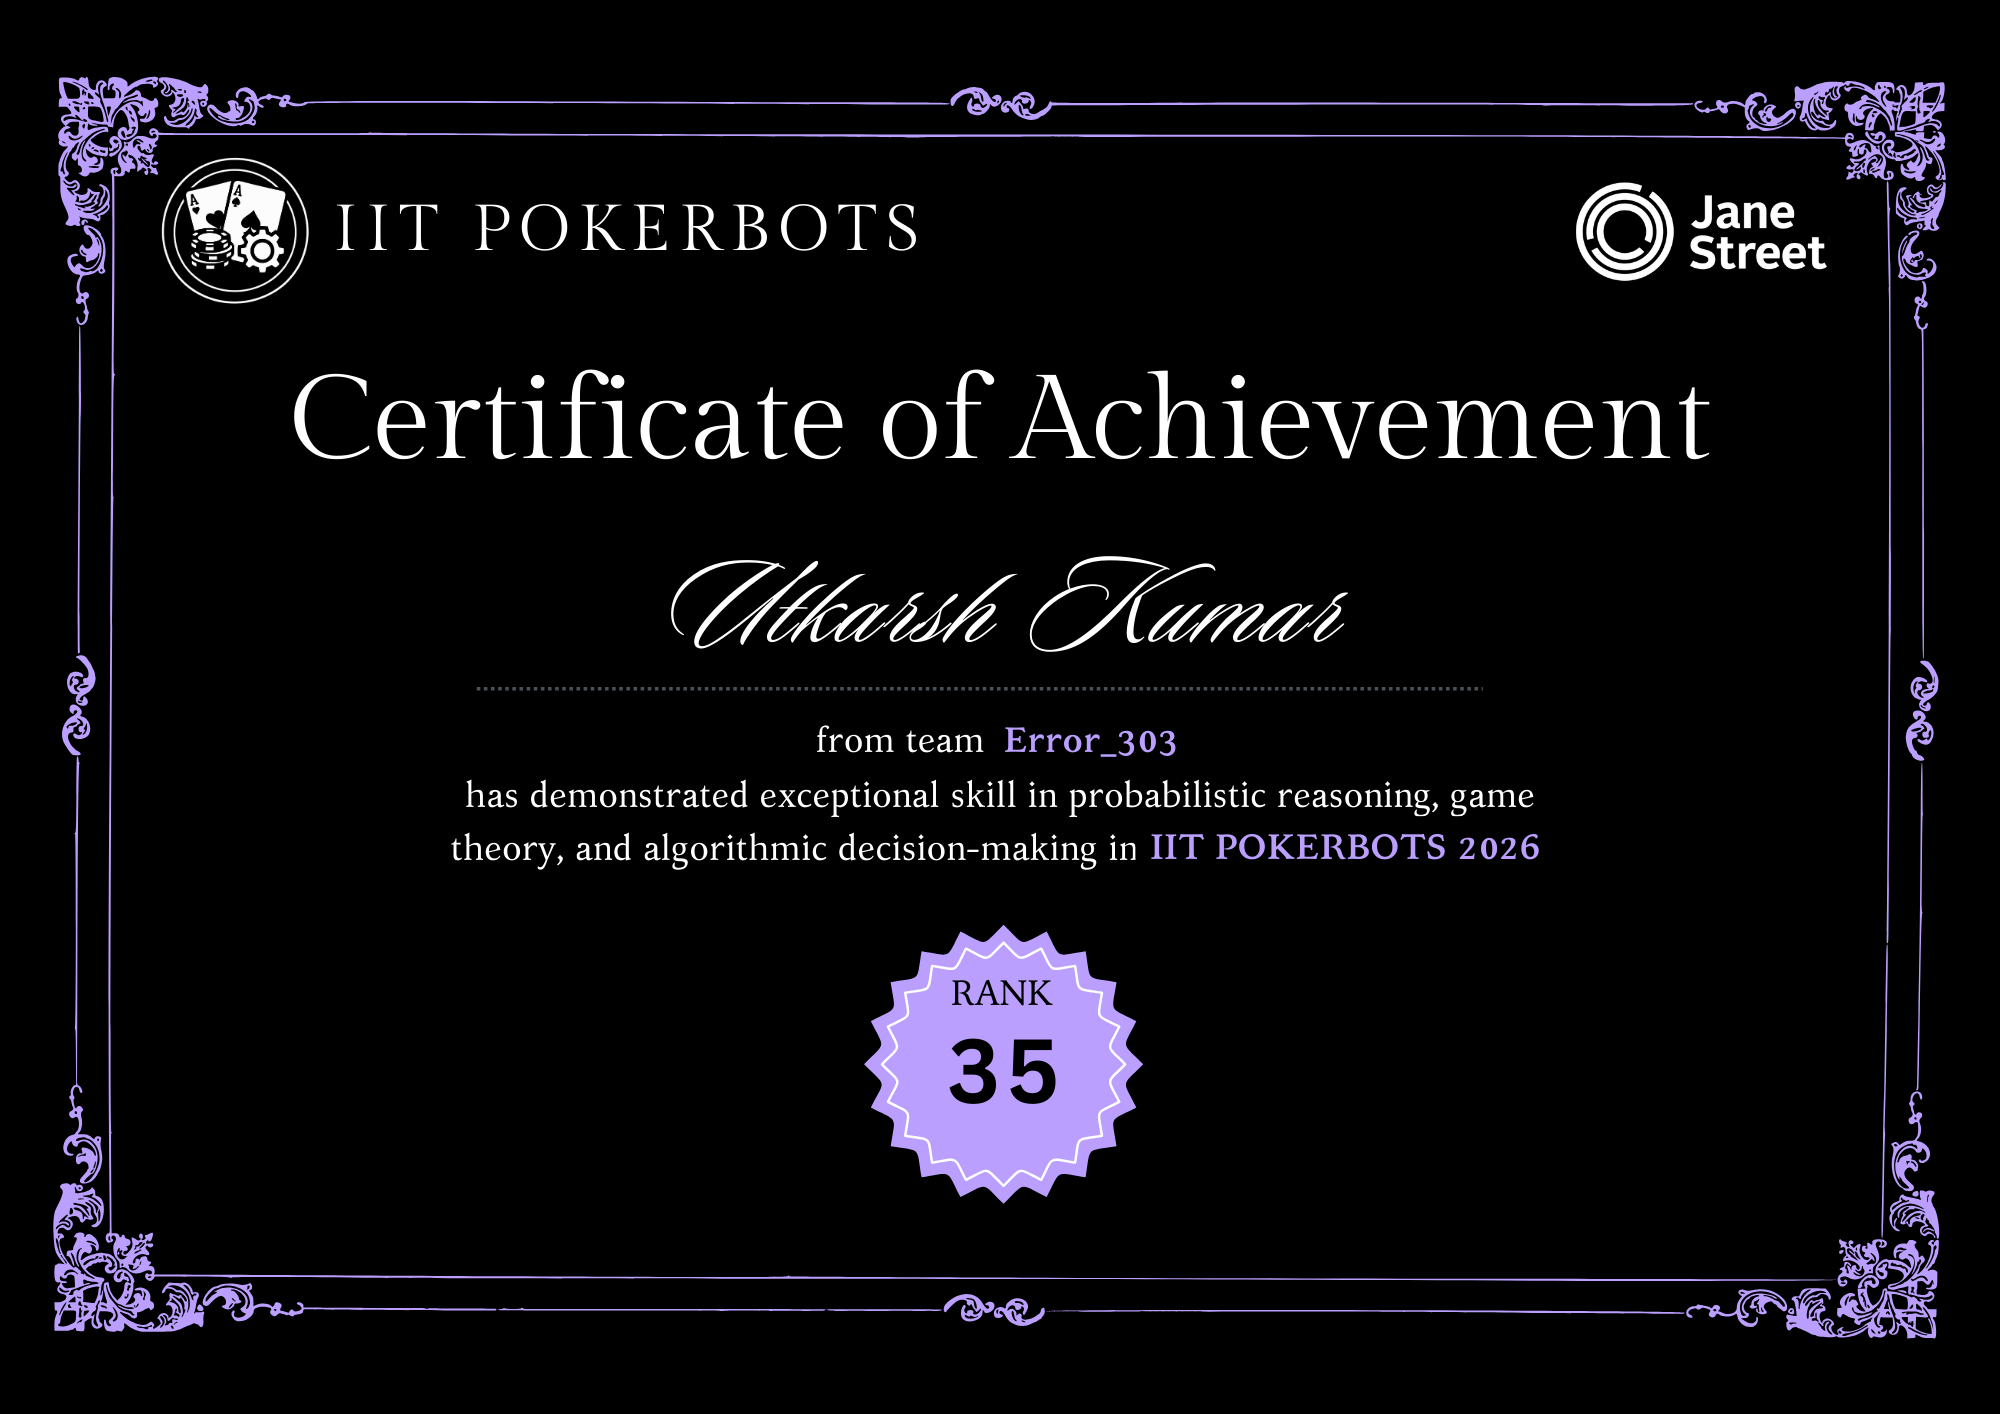
\includegraphics[width=\textwidth]{imgs/pokerbots.png}
\caption{IIT Pokerbots 2026 Certificate}
\end{minipage}
\end{figure}

\vspace{-1cm}
\chapter*{Competition - Codefest 2026}

I took part in multiple demanding coding contests and problem-solving events which were organized by Intercollegiate Informatic and Competitive Programming Camp (IICPC) for their Codefest 2026 event. The competition took place in two major competition rounds which were:

\begin{itemize}[noitemsep, topsep=0pt]
    \item \textbf{Global Prelims:} A intensive offline algorithmic contest happened on \href{https://codefest.iicpc.com/}{31 Jan 2026}.
    \item \textbf{Global Regionals:} Advanced algorithmic and system design challenges for participants on \href{https://codefest.iicpc.com/}{15 Mar 2026}.
\end{itemize}

I proved my technical expertise by achieving a \textbf{Rank of 483} in the CodeFest'26 Global Prelims. I progressed to the Regionals where I achieved \textbf{Rank 291} in the CodeFest Global Regionals 2026.

\vspace{2em}

\noindent
\begin{minipage}{0.4\textwidth}
    \centering
    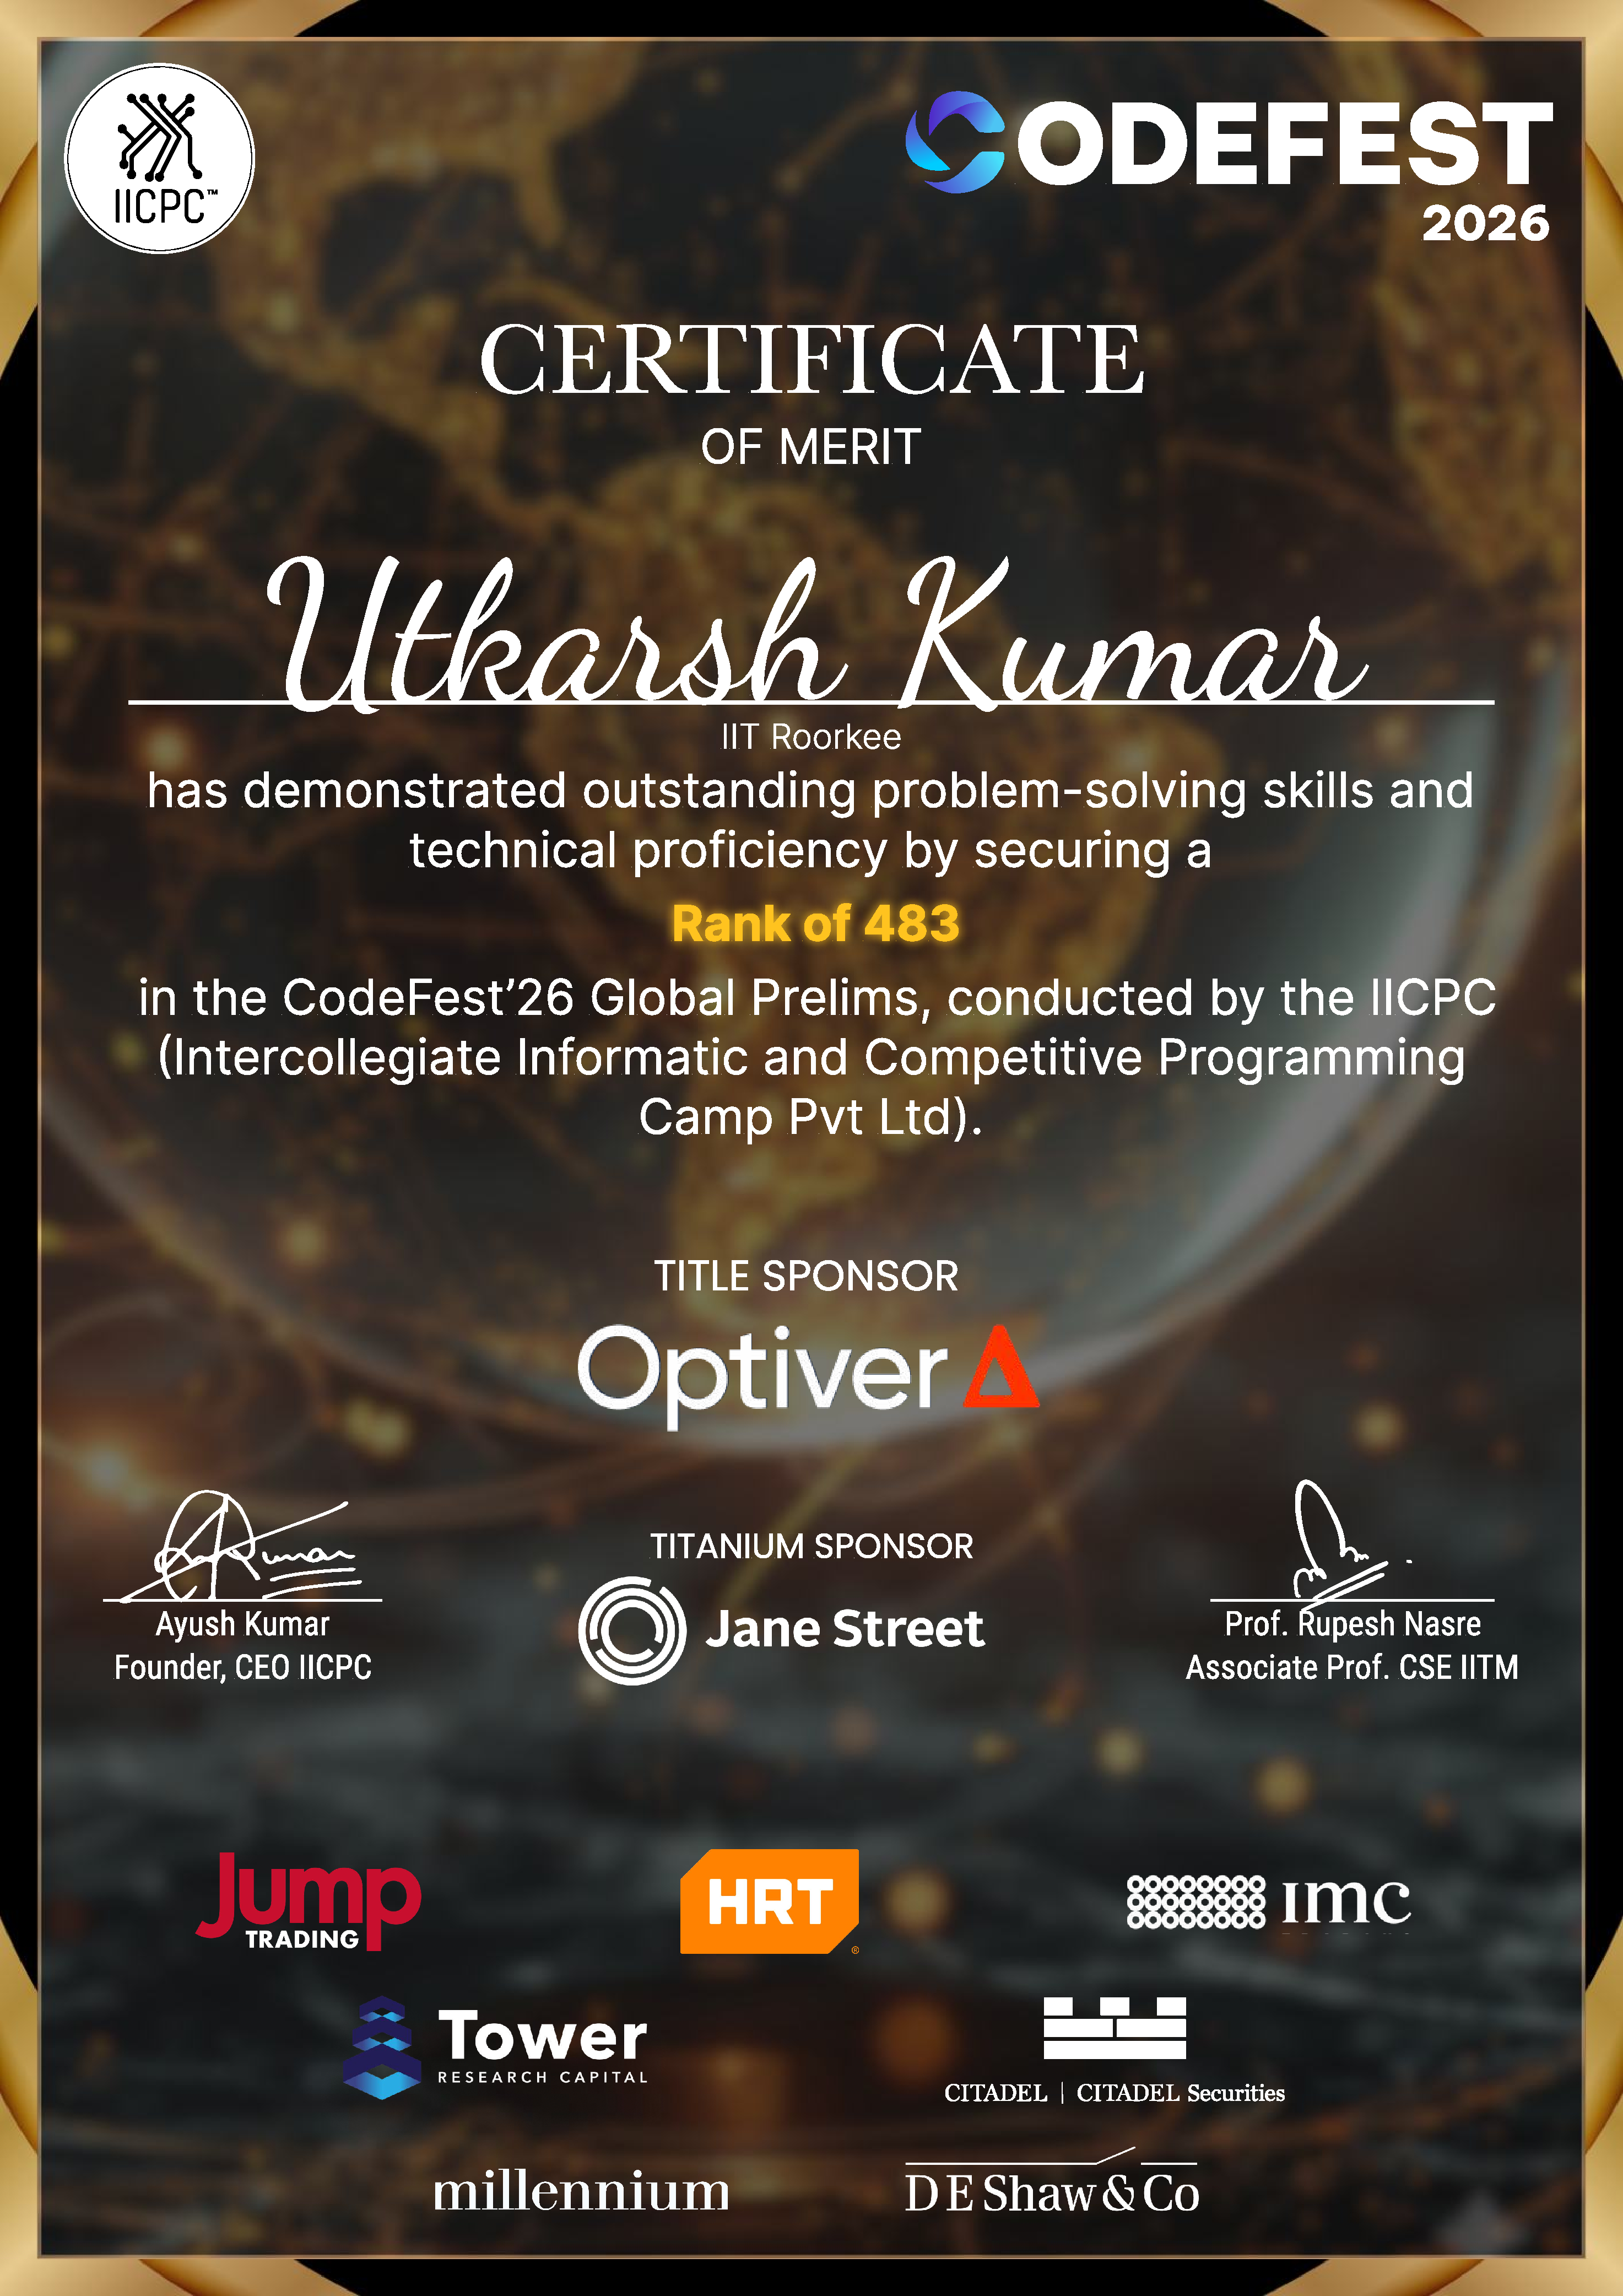
\includegraphics[page=1,height=0.3\textheight,keepaspectratio]{imgs/prelims.pdf}
    \captionof{figure}{Codefest 2026 Prelims Certificate}
\end{minipage}
\hspace{0.04\textwidth}
\begin{minipage}{0.55\textwidth}
    \centering
    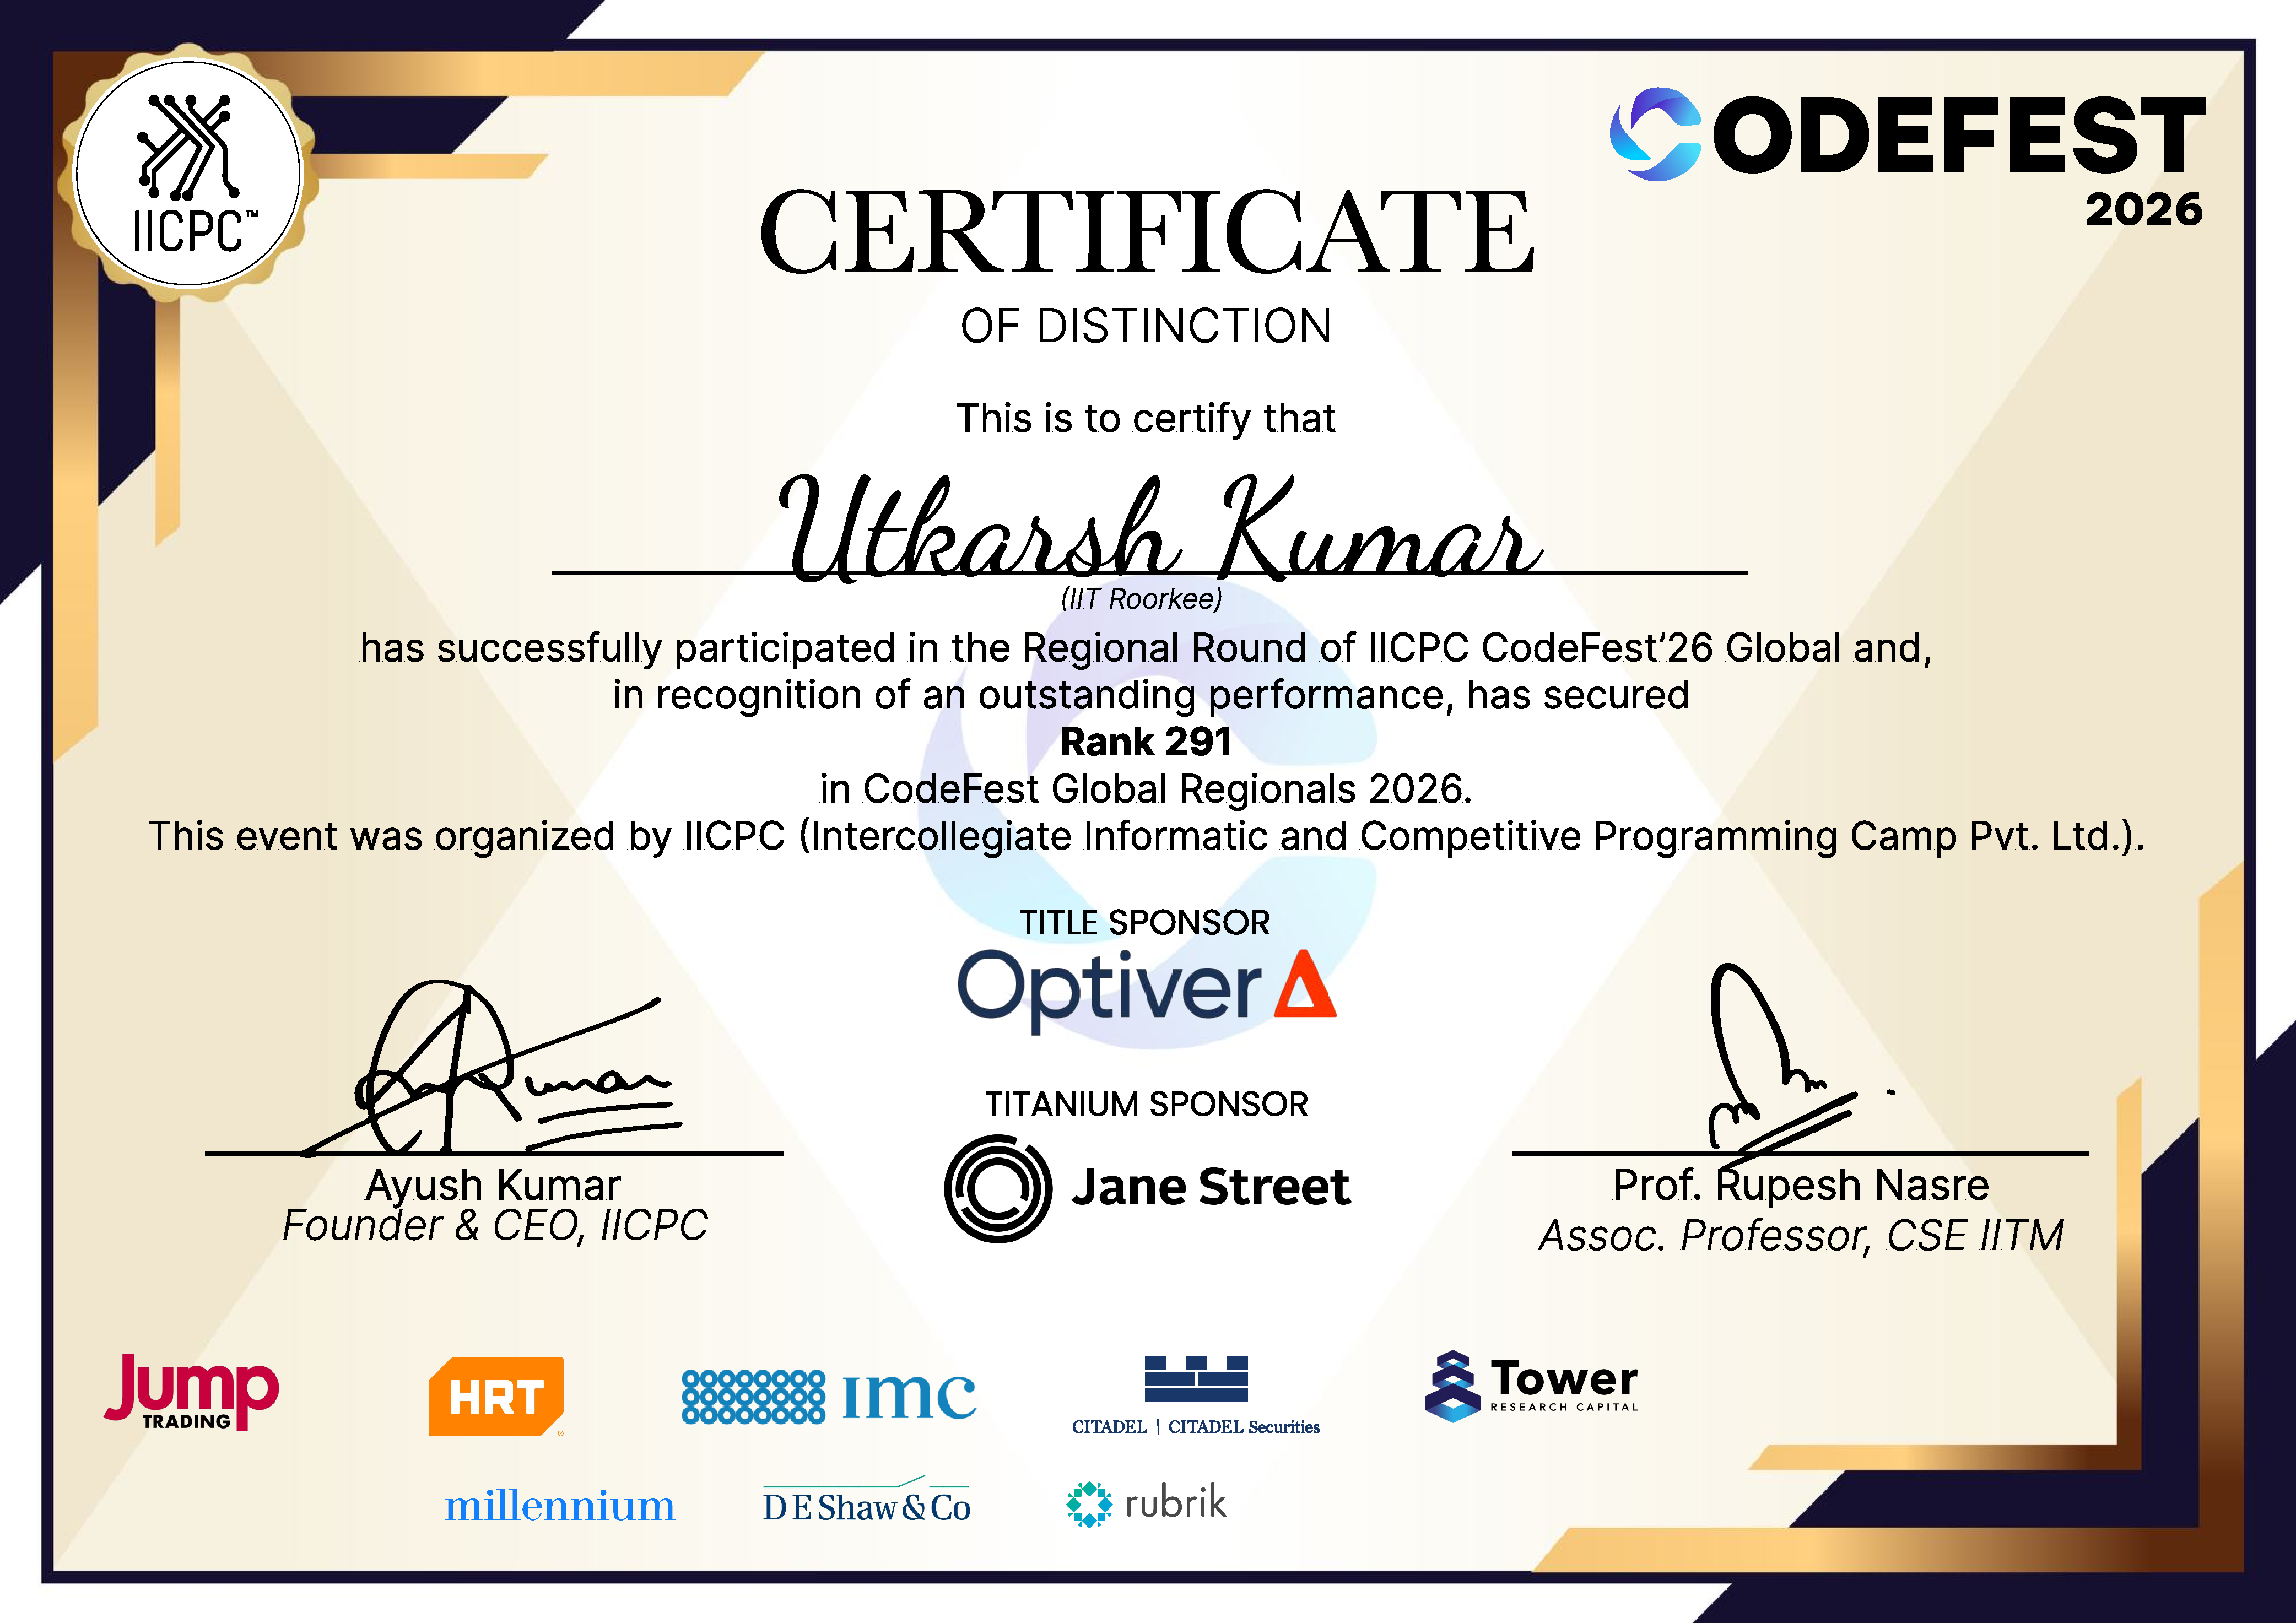
\includegraphics[page=1,width=\textwidth]{imgs/regional.pdf}
    \captionof{figure}{Codefest 2026 Regionals Certificate}
\end{minipage}

\newpage
\chapter*{Course - Introductory Options}

\begin{figure}[htbp]
\centering
\begin{minipage}{0.45\textwidth}
I successfully completed the Introductory Options course of \textbf{one week} which the Finance and Economics Club at IIT Guwahati offered in January 2026. The course provided a strong theoretical and practical foundation in financial derivatives, with a focus on real-world applications.

\vspace{1em}
The curriculum covered options pricing models, risk management techniques, and hedging strategies, along with the implementation of various trading approaches used in modern financial markets. The study program required students to learn market behavior together with quantitative methods which they needed for making successful decisions.

\end{minipage}
\hfill
\begin{minipage}{0.5\textwidth}
\centering
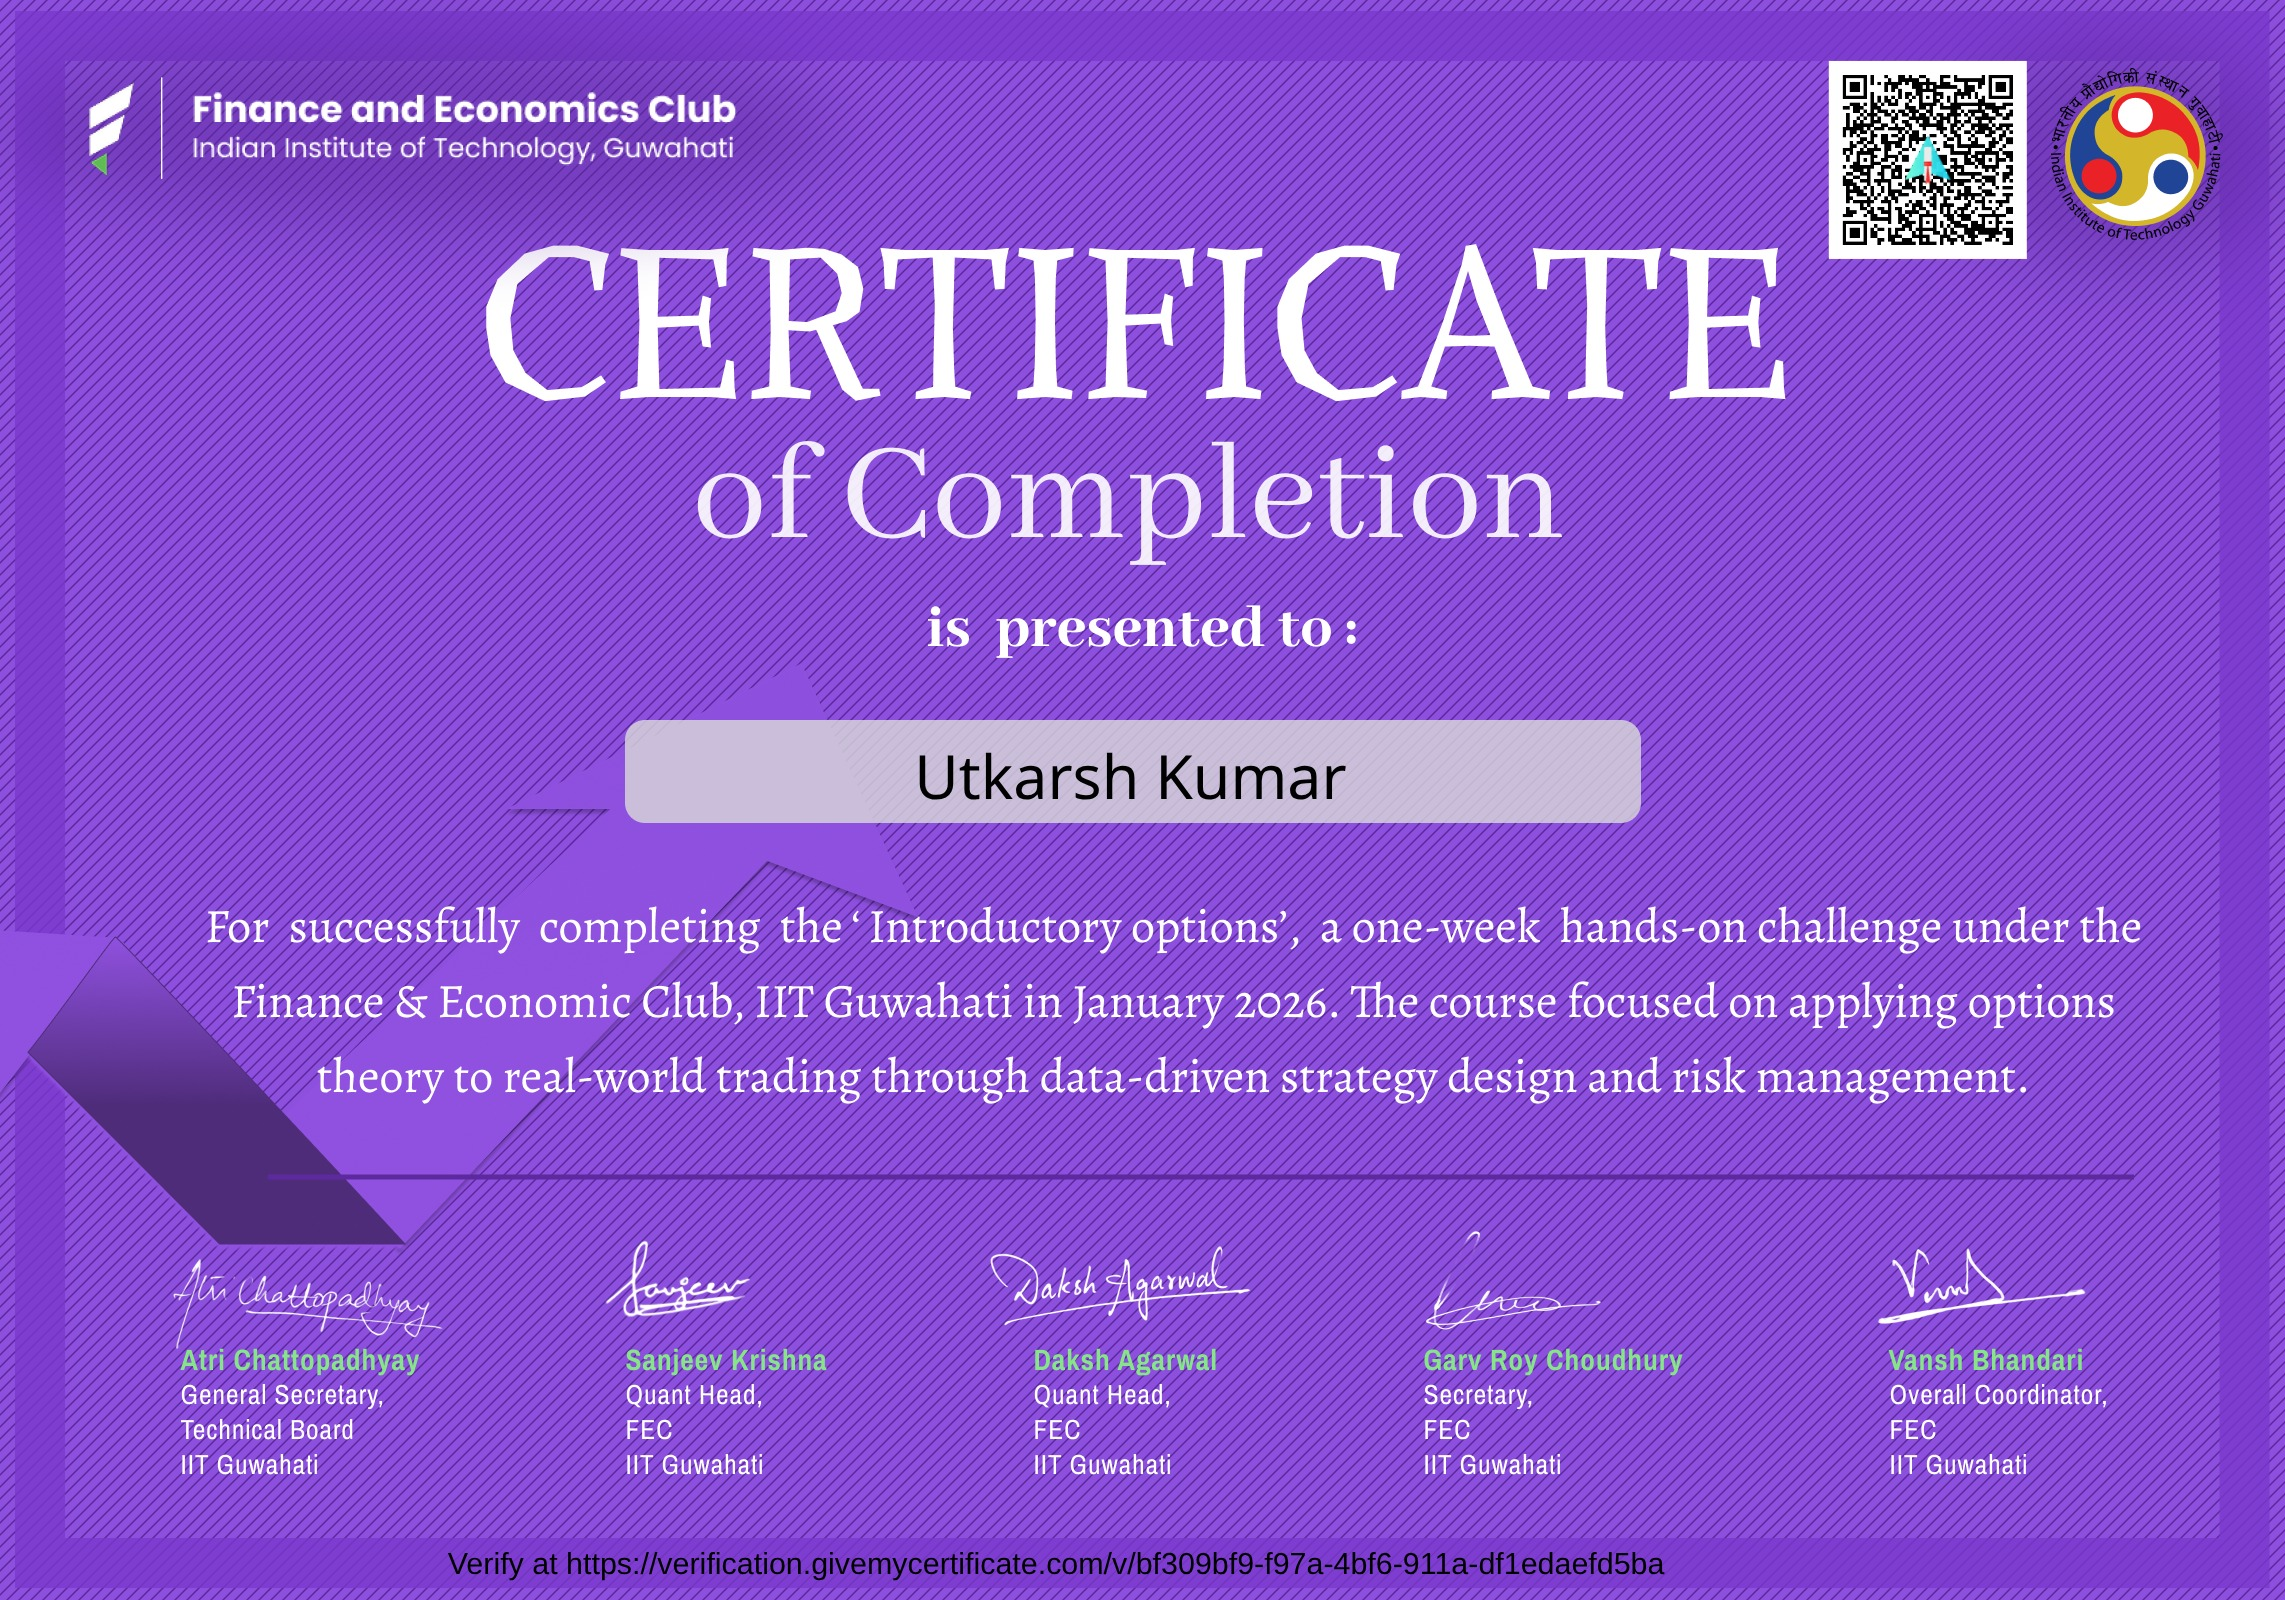
\includegraphics[width=\textwidth]{imgs/options.png}
\caption{Introductory Options Certificate}
\end{minipage}
\end{figure}


\chapter*{Course - Corporate Finance Essentials}

\begin{figure}[htbp]
\centering
\begin{minipage}{0.45\textwidth}
I also achieved completion of the \textbf{two-week} Corporate Finance Essentials course which the Finance and Economics Club (FEC) at IIT Guwahati presented in February 2026. The course delivered complete knowledge about corporate finance principles together with their real-world applications.

\vspace{1em}

The main subjects of study included investment assessment methods and financial market operations and time value of money and corporate valuation methods. The program focused on teaching students how to think analytically while using quantitative methods in financial decision-making and business strategy development.
\end{minipage}
\hfill
\begin{minipage}{0.5\textwidth}
\centering
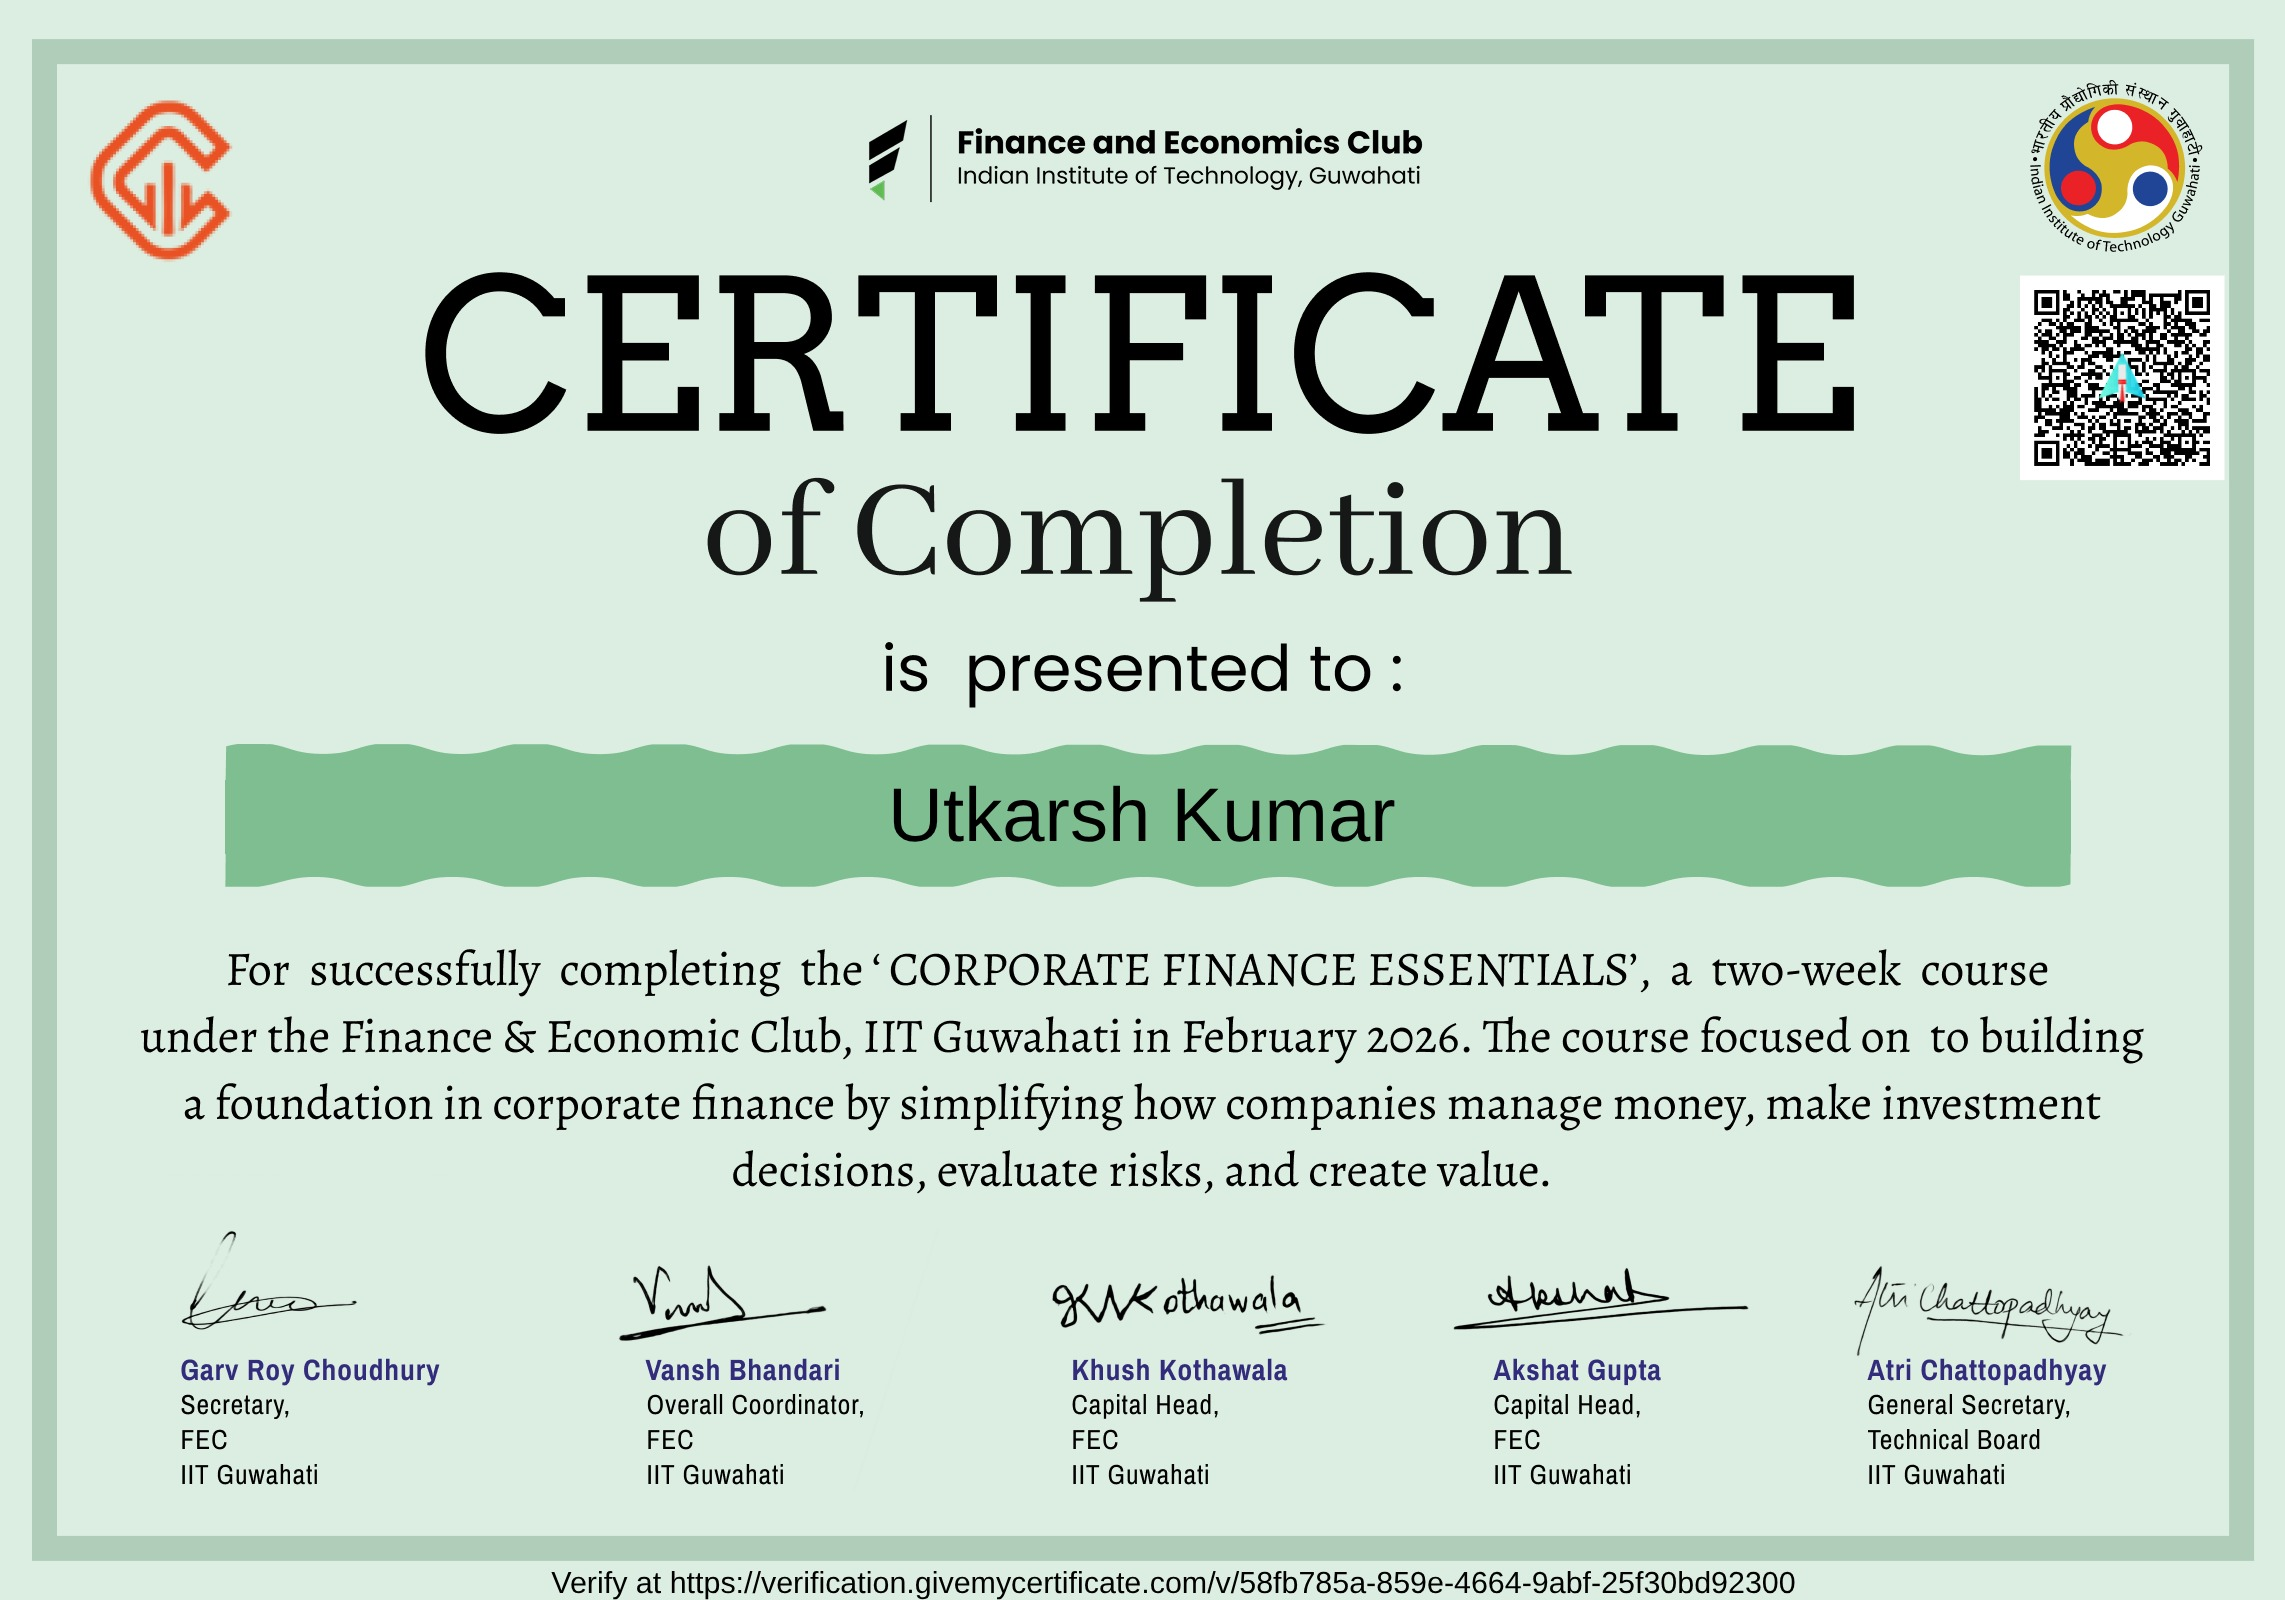
\includegraphics[width=\textwidth]{imgs/corporate.png}
\caption{Corporate Finance Essentials Certificate}
\end{minipage}
\end{figure}

\vspace{-0.6cm}

\chapter*{Declaration}

I hereby declare that this report titled \textbf{``\ttitle''} is a record of my own work carried out as part of the Professional Development Program. All information presented in this report is based on my personal participation, learning, and achievements during the program.

\vspace{1em}
\noindent
\begin{tabular}{p{0.6\textwidth} p{0.35\textwidth}}
& \hfill \textbf{Utkarsh Kumar} \\
Date: April, 2026  & \hfill 23114101 \\
\end{tabular}

\clearpage

